\documentclass[a4paper,11pt]{article}

\usepackage{babel}
\usepackage{graphicx}
\usepackage{amsmath, amssymb}
\usepackage{ngerman}
\usepackage{verbatim}
\usepackage{mathtools}
\usepackage{makecell}
\usepackage{hyperref}
\usepackage{tikz}


%margins
\addtolength{\oddsidemargin}{-0.75in}
\addtolength{\evensidemargin}{-0.75in}
\addtolength{\textwidth}{1in}
\addtolength{\topmargin}{-.5in}
\addtolength{\textheight}{1.0in}


%annotation above equals
\newcommand\eqthreei{\overset{\mathclap{\scriptscriptstyle (iii)}}{=}}
\newcommand\eqoneone{\overset{\mathclap{\scriptscriptstyle (1.1)}}{=}}
\newcommand\eqonetwo{\overset{\mathclap{\scriptscriptstyle (1.2)}}{=}}
\newcommand\eqonethree{\overset{\mathclap{\scriptscriptstyle (1.3)}}{=}}
\newcommand\eqonefive{\overset{\mathclap{\scriptscriptstyle (1.5)}}{=}}
\newcommand\eqonei{\overset{\mathclap{\scriptscriptstyle (i)}}{=}}
\newcommand\eqasb{\overset{\mathclap{\scriptscriptstyle A \subset B}}{=}}
\newcommand\geqonei{\overset{\mathclap{\scriptscriptstyle (i)}}{\geq}}
\newcommand\Raonethree{\overset{\mathclap{\scriptscriptstyle (1.3)}}{\Rightarrow}}
\newcommand\stw{\overset{\mathclap{\scriptscriptstyle (2.1.2)}}{=}}
\newcommand\Btuwon{\overset{\mathclap{\scriptscriptstyle (B.2.1)}}{=}}
\newcommand\Dtuwon{\overset{\mathclap{\scriptscriptstyle (D.2.1)}}{=}}
\newcommand\fover{\overset{\mathclap{\scriptscriptstyle (f)}}{=}}

\newcommand\eqsigmaadd{\overset{\mathclap{\scriptscriptstyle (\sigma\text{-Add.})}}{=}}
\newcommand\eqthreetwog{\overset{\mathclap{\scriptscriptstyle (Satz 3.2(g))}}{=}}
\newcommand\impthreetwog{\overset{\mathclap{\scriptscriptstyle (Satz 3.2(g))}}{\Rightarrow}}



%unused
%Falls die Ereignisse $A_1,A_2,\dots$ eine Zerlegung von $\Omega$ bilden, d.h. falls gilt $A_1,A_2,\dots$ sind paarweise disjunkt und $A_1 \cup A_2 \cup \dots = \Omega$, 
%dann gilt für jedes Ereignis B mit $P(B) = P(B\cap A_1) + P(B\cap A_2) + \dots$, denn: 
%$P(B)=P(B\cap\Omega)=P(B\cap(A_1\cup A_2\cup\dots))=P((B\cap A_1)\cup(B\cap A_2)\cup\dots)$ (es gilt: $(B\cap A_i)$ und $(B\cap A_j)$ sind paarweise disjunkt für $i\neq j$.) 



\begin{document}

\title{\Huge{\textbf{Statistik - SoSe 2025}}}
\author{}
\date{}
\maketitle
\tableofcontents

\part{Wahrscheinlichkeitsrechnung}

\section{Grundbegriffe}

\subsection{Ergebnismenge und Ereignisse}
Alle möglichen Ergebnisse eines Zufallsexperiments fasst man zur Ergebismenge $\Omega$ (Groß Omega) zusammen.

\vspace{6pt}
\noindent\textbf{Bsp. 1.1:} Zweimaliges Werfen eines Würfels
\begin{align*} 
    \Omega &= \{(1,1),(1,2),\dots,(1,6),(2,1),\dots,(6,6)\} \\
        &= \{(i,j): 1\leq i\leq 6,1\leq j\leq 6\}\\
        &=\{1,\dots,6\}\times\{1,\dots,6\}=\{1,\dots,6\}^2
\end{align*}

\vspace{6pt}
\noindent\textbf{Bsp. 1.2:} Ziehung der Lottozahlen (6 aus 49)
\[\Omega = \{(\omega_1,\dots,\omega_6):\omega_i \in \{1,2,\dots,49\}, 1\leq i\leq6, \omega_1 < \omega_2 <\dots<\omega_6\}\]

\vspace{6pt}
\noindent\textbf{Bsp. 1.3:} Verkaufszahlen. Ein Laden erhält morgens 3 Tageszeitungen $Z_1,Z_2,Z_3$, und zwar 100 bzw. 200 bzw. 250 Stück. Die verkauften Anzahlen sind dann als Ergebis eines Zufallsexperiments zu interpretieren.
\begin{align*}
    \Omega &= \{(\omega_1,\omega_2,\omega_3): \omega_1 \in \{0,1,\dots,100\}, \omega_2 \in \{0,1,\dots,200\}, \omega_3 \in \{0,1,\dots,250\}\} \\
    &= \{0,1,\dots,100\}\times\{0,1,\dots,200\}\times\{0,1,\dots,250\}
\end{align*}

\vspace{6pt}
\noindent Ein Ereignis ist eine Teilmenge der Ergebnismenge. Ereignisse werden zunächst verbal beschrieben 
und lassen sich dann als Teilmengen von $\Omega$ auffassen.

\vspace{6pt}
\noindent\textit{In Bsp. 1.1:}
\begin{itemize}
    \item[-] Ereignis E: Augensumme ist 10; zugeordnete Teilmenge von $\Omega: E = \{(4,6),(5,5),(6,4)\}$
    \item[-] E: Pasch; $E = \{(1,1),(2,2),(3,3),(4,4),(5,5),(6,6)\}$
    \item[-] E: mindestens eine 6; $E = \{(6,1),(6,2),\dots(6,6),(5,6),\dots,(1,6)\}$
\end{itemize}

\vspace{6pt}
\noindent\textit{In Bsp. 1.3:}
\newline Ereignis A: Von jeder der 3 Zeitungen werden mindestens 50 Stück verkauft
\newline Teilmenge: $A = \{(\omega_1,\omega_2,\omega_3)\in\Omega:\omega_1\leq50,\omega_2\leq50,\omega_3\leq50\}=\{50,51,\dots,100\}\times\{50,51,\dots,200\}\times\{50,51,\dots,250\}$

\vspace{6pt}
\noindent Ist $\omega\in\Omega$ das betrachtete Ergebnis eines Zufallsexperiments und ist $E\subset\Omega$ ein Ereignis, so sagt man \textit{E ist eingetreten}, falls $\omega\in E$ und \textit{E ist nicht eingetreten}, falls $\omega\notin E$.

\noindent Übertrage Begriffe der Mengenlehre auf das zufällige Eintreten von Ereignissen. (Dies wird durch die Zuordnung \textit{Ereignis} $\Leftrightarrow$ \textit{Teilmenge von $\Omega$} möglich.)

\vspace{6pt}
\begin{center}
\noindent\begin{tabular}{|c|c|}
\hline
\textbf{Mengenschreibweise} & \textbf{Interpretation für Ereignisse}\\
\hline
$A=\Omega$ & \makecell{A ist ein sicheres Ereignis \\ \small{(A tritt sicher ein)}}\\
\hline
$A=\emptyset$ & \makecell{A ist ein unmögliches Ereignis \\ \small{(A tritt nicht ein)}}\\
\hline
\makecell{$A^c = \{\omega\in\Omega, \omega\notin A\}$ \\ $\bar{A}=A^c$ \footnotesize{(andere Schreibweise)}}  & \makecell{Komplementärereignis zu A \\ \small{(A tritt nicht ein)}}\\
\hline
$A\cap B$  & \makecell{A geschnitten B. \\ \small{(A und B treten ein.)}} \\
\hline
$\bigcap_{i=1}^{n}A_i = A_1\cap\dots\cap A_n$ & \makecell{Durchschnitt der Ereignisse $A_1,\dots,A_n$ \\ \small{(Jedes dieser Ereignisse $A_1,\dots,A_n$ tritt ein.)}}\\
\hline
$A\cap B = \emptyset$ & \makecell{A und B sind disjunkt. \\ \small{(A und B treten sicher nicht zusammen ein.)}} \\
\hline
$A\cup B$ & \makecell{Vereinigung von A und B. \\ \small{(A oder B tritt ein. \glqq Oder\grqq\  ist nicht ausschließend.)}} \\
\hline
$\bigcup_{i=1}^{n}A_i = A_1\cup\dots\cup A_n$ & Mindestens eines der Ereignisse tritt ein. \\
\hline
$A\subset B$ & \makecell{Implikation: \\ \small{Aus dem Eintreten von A folgt das Eintreten von B.}} \\
\hline
$A\backslash B = A\cap B^c$ & A tritt ein, aber B tritt nicht ein. \\
\hline
\end{tabular}
\end{center}

\vspace{2pt}
\noindent Einelementige Teilmengen $\{\omega\}\subset\Omega$ (die nur einen Punkt enthalten) nennt man Elementarereignisse.

\vspace{6pt}
\noindent\textbf{Bsp. 1.4:} Einmaliges Werfen eines Würfels; $\Omega = \{1,\dots,6\}$
\newline Ereignis $A$: \glqq Augenzahl ist gerade\grqq\ $\Rightarrow$ $A=\{2,4,6\}$, Ereignis $B$: \glqq Augenzahl ist mindestens 4\grqq\ $\Rightarrow B=\{4,5,6\}$
\newline\noindent\begin{tabular}{c|c}
Schreibweise & Interpretation\\
\hline
$A^c = \{1,3,5\}$ & Augenzahl ist ungerade\\
$B^c = \{1,2,3\}$ & Augenzahl ist kleiner als 4\\
$A\cap B = \{4,6\}$ & Augenzahl ist gerade und mind. 4\\
$A\cup B = \{2,4,5,6\}$ & Augenzahl ist gerade oder mind. 4\\
$B\backslash A = B\cap A^c = \{4,5,6\}\cap\{1,3,5\}=\{5\}$ & Augenzahl ist mind. 4, aber nicht gerade.\\
$A\backslash B = A\cap B^c = \{1,3,5\}\cap\{4,5,6\}=\{1,3\}$ & Augenzahl ist nicht gerade, aber mind. 4\\
\end{tabular}

\subsubsection{Rechenregeln für Mengen}
\noindent Für beliebige Mengen A,B,C gilt:
\begin{itemize}
    \item Kommutativgesetze: $A\cup B = B\cup A$, $A\cap B = B\cap A$
    \item Assoziativgesetze: $A\cup(B\cup C)=(A\cup B)\cup C$; $A\cap(B\cap C)=(A\cap B)\cap C$
    \item Distributivgesetze: $A\cup(B\cap C) = (A\cap B) \cup (B\cap C); (A\cap B)\cup C = (A\cup C)\cap (B\cup C)$
    \item Komplement: $(A^c)^c = A$
    \item De Morgansche Regeln: $(A\cup B)^c = A^c\cap B^c, (A\cap B)^c = A^c\cup B^c$
\end{itemize}
Hinweis: Um das Komplement verwenden zu können benötigt man eine bestimmte Obermenge.

\vspace{6pt}
\noindent Allgemeiner: Für beliebige $A_1,\dots,A_n$ und B gilt:
\begin{itemize}
    \item Kommutativ- und Assoziativgesetze gelten, da die Reihenfolge keine Rolle spielt.
    \item $(\bigcup_{i=1}^{n}A_i)\cap B = \bigcup_{i=1}^{n}(A_i\cap B)$
    \item $(\bigcap_{i=1}^{n}A_i)\cup B = \bigcap_{i=1}^{n}(A_i\cup B)$
    \item $(\bigcup_{i=1}^{n}A_i)^c = \bigcap_{i=1}^{n}A_i^c$,$(\bigcap_{i=1}^{n}A_i)^c = \bigcup_{i=1}^{n}A_i^c$
    \item Für beliebige Mengen A,B gilt $A\subset B \Leftrightarrow A^c\supset B^c$
\end{itemize}

\vspace{6pt}
\noindent Beweis für $(\bigcup_{i=1}^{n}A_i)^c = \bigcap_{i=1}^{n}A_i^c$, wobei die Komplemente bzgl. $\Omega$ gebildet werden.
\newline Für jedes $\omega\in\Omega$ gilt:
\begin{align*}
\omega\in(\bigcup_{i=1}^{n}A_i)^c &\Leftrightarrow \omega\notin\bigcup_{i=1}^{n}A_i\\
&\Leftrightarrow \omega\text{ ist in keiner der Mengen } A_1,\dots,A_n\text{ enthalten.}\\ 
&\Leftrightarrow \omega\in A_1^c\ \text{und}\ \omega\in A_2^c\ \text{und}\dots\text{und}\ \omega\in A_n^c\\
&\Leftrightarrow \omega\in\bigcap_{i=1}^{n}A_i^c\\
\end{align*}

\subsection{Wahrscheinlichkeitsmaße}

\noindent\textbf{Def. 1.1:} Es sei $\Omega\neq\emptyset$ einer Ergebnismenge. 
Eine für alle Ereignisse $A\subset\Omega$ definierte reelwertige Funktion P heißt \textbf{Wahrscheinlichkeitsmaß} auf $\Omega$ falls sie die folgenden Axiome der Wahrscheinlichkeitsrechnung erfüllt:
\begin{itemize}
    \item[(i)] $P(A)\geq0$ für alle Ereignisse $A<\Omega$
    \item[(ii)] $P(\Omega)=1$
    \item[(iii)] $\sigma$-Additivität: $P(A_1 \cup A_2\cup\dots) = P(A_1)+P(A_2)+\dots$ gilt für jede endliche oder unendliche Folge von paarweise disjunkten Ereignissen $A_1,A_2,\dots\subset\Omega$    
\end{itemize}

\noindent P(A) heißt \textit{Wahrscheinlichkeit} von A (probability). 
($\Omega,P$) heißt \textit{Wahrscheinlichkeitsmodell} für das Zufallsexperiment. 
(i)-(iii) heißen \textit{Axiome der Wahrscheinlichkeitsrechnung} oder \textit{Kolmogorov-Axiome}.

\vspace{6pt}
\noindent\textbf{Bsp. 1.5:} Zweimaliges Werfen eines Würfels.
\newline $\Omega = \{(i,j):1\leq i\leq6,1\leq j\leq6\}$
\newline Für $A\subset\Omega$ sei $P(A)=\frac{|A|}{|\Omega|}=\frac{|A|}{36}$, wobei $|A|$ = Anzahl der Elemente von A. Dann ist P ein W-Maß, denn P ist reelwertig
\newline (i) $P(A) \geq0$ für alle $A\subset\Omega$
\newline (ii) $P(\Omega)=\frac{|\Omega|}{|\Omega|}=1$
\newline (iii) Sind $A_1,\dots,A_n$ paarweise disjunkte Teilmengen von $\Omega$, so ist $|\bigcup_{i=1}^{n}A_i| = \sum_{i_1}^{n}|A_n|$, 
also $P(\bigcup_{i=1}^{n}A_i) = \frac{|\bigcup_{i=1}^{n}A_i|}{|\Omega|} = \frac{\sum_{i_1}^{n}|A_n|}{|\Omega|} = \sum_{i=1}^{n}\frac{|A_i|}{|\Omega|} = \sum_{i=1}^{n}P(A_i)$.

\vspace{2pt}
\noindent Für jede unendliche Folge von paarweise disjunkten Teilmengen $A_1,\dots,A_n$ von $\Omega$ existiert ein $N\in\mathbb{N}$, so dass $A_i=\emptyset$ für alle $i>N$, da $\Omega$ endlich ist.
Es gilt also:
\newline $\Rightarrow P(\bigcup_{i=1}^{\infty}A_i)=P(\bigcup_{i=1}^{\mathbb{N}}A_i)$
\newline $\Rightarrow P(\sum_{i=1}^{\mathbb{N}}A_i)=P(\sum_{i=1}^{\infty}A_i)$
\newline $P(A_i)=P(\emptyset)=\frac{|\emptyset|}{|\Omega|}=0\ \text{für alle}\ i\notin\mathbb{N}$
\newline Für das Ergebnis A: \glqq Augensumme ist 10\grqq, also $A=\{(4,6),(5,5),(6,4)\}$ ergibt sich $P(A_i)=\frac{|A|}{|Omega|}=\frac{3}{36}=\frac{1}{12}$.
\newline Für das Ergebnis B: \glqq Pasch\grqq, also $B=\{(1,1),(2,2),\dots,(6,6)\}$ ergibt sich 
\newline$P(A)=\frac{|A|}{|Omega|}=\frac{6}{36}=\frac{1}{6}$.


\vspace{9pt}
\noindent Ist allgemeiner $\Omega \neq \emptyset$ eine beliebige endliche Menge und haben alle Ergebnisse 
(genauer: alle Elementarereignisse) dieselbe Wahrscheinlichkeit, dann folgt aus Axiomen (ii) und (iii)

\[ P(\{w\})=\frac{1}{|\Omega|} \]

\noindent und daher wegen Axiom (iii) \[ P(A)=\frac{|A|}{|\Omega|} \]

\noindent Also \[ P(A)=\frac{\text{Anzahl der Ergebnisse in A}}{\text{Anzahl aller m"oglichen Ergebnisse}} \] 

\noindent P(A) heißt \textit{Laplace-Wahrscheinlichkeit} von A.

\vspace{6pt}
\noindent\textbf{Bsp. 1.6} Roulette.
Wenn $\Omega = \{0,1,...,36\} $ ist die W'keit, dass eine ungerade Zahl fällt, $P(\{1,3,5,...,35\})=\frac{|\{1,3,5,...,35\}|}{|\Omega|} = \frac{18}{37}$.

\noindent\ Grundlegendes Prinzip des Zählens ... was heißt das?

\vspace{6pt}
\noindent\textbf{Multiplikationsregel:} Betrachte k Aufgaben. Nimm an, die 
1. Aufgabe kann auf $n_1$ Arten erledigt werden; danach kann die 
2. Aufgabe auf $n_2$ Arten erledigt werden;...; danach kann die 
k-te Aufgabe erledigt werden. (Annahme: $n_1,n_2,...,k$ sind unabhängig.) 
\newline Die Anzahl der Möglichkeiten, alle k Aufgaben zu erledigen, ist $n_1*n_2*...*k$

\vspace{6pt}
\noindent\textbf{Bsp. 1.7:} Eine faire Münze wird n-mal geworfen. 
Ergebnisse sind Folgen von Kopf(K) und Zahl(Z) der Länge n: $\Omega = \{(x_1,...,x_n): x_i\in\{K,Z\}, i = 1,...,n\}$. 
Verwende Laplace-Wahrscheinlichkeiten: $P(A)=\frac{|A|}{|\Omega|}=\frac{|A|}{2^n}$ für alle $A\in\Omega$.
Wie groß ist die Wahrscheinlichkeit von $A_j$: \glqq K fällt im j-ten Wurf zum 1. Mal\grqq?
\[A_j = \{x_1,...,x_n\}: x_i=Z \text{ für } 1 \leq i \leq j-1; x_j=K; x_i \{K,Z\} \text{ für } j+1 \leq i \leq n\]
\[A_j = 1^{j-1}\cdot 1\cdot 2^{n-j}=2^{n-j} \rightarrow P(A_j) = \frac{|A_j|}{|\Omega|}= \frac{2^{n-j}}{2^{n}}\]

\noindent\textbf{Bsp. 1.8:} Geburtstagsproblem.
W'keit, dass von k Personen 2 oder mehr am selben Tag im Jahr Geburtstag haben?
$2 \leq k \leq 365$ ohne (29.2) und verwende Laplace-W'keiten mit $\Omega=\{x_1,...,x_k\}: x_i \in \{1,...,365\}, i=1,...,k$, also 
$P(A)=\frac{|A|}{|\Omega|}=\frac{|A|}{365}$ für alle $A\subset\Omega$.
$\text{Sei }B=\{(x_1,...,x_k) \in\Omega: \text{mind. 2 der } x_i \text{ stimmen überein}\}$
\begin{align*}
    |B^c| &= \{(x_1, \dots ,x_k) \in \Omega: x_i \neq x_j \text{ für }i \neq j\} \\
    &= 365 \cdot 364 \cdot 363 \cdot\dots\cdot (365-k+1) \\
    &= \prod_{i=0}^{k-1}(365-i) \\
    \rightarrow P_k = P(B) &= \frac{|\Omega| - |B^c|}{|\Omega|} = 1 - \frac{1}{365}\cdot \prod_{i=0}^{k-1}(365-i) \\
    &= 1 - \prod_{i=0}^{k-1}(1-\frac{i}{365}) \text{           z.B. } P_{30} = 0,705
\end{align*}

\subsubsection{Rechenregeln für Wahrscheinlichkeitsmaße}

\begin{itemize}
    \item[1.1] $P(A^c)=1-P(A)$, denn $1=P(\Omega)=P(A\cup A^c) \eqthreei P(A) + P(A^c) \Rightarrow (1.1)$
    \item[1.2] $P(\emptyset)=0$, denn $P(\emptyset)=P(\Omega^c) \eqoneone 1-P(\Omega) = 1-1 = 0$
    \item[1.3] Falls $A\subset B$, dann $P(B \backslash A)=P(B)-P(A)$, denn: Falls $A\subset B$, dann $B=B\cap (A\cup A^c) = (B\cap A) \cup (B \cap A^c) \eqasb A\cup (B \cap A^c) \Rightarrow P(B) \eqthreei P(A) + P(B\cap A^c) = P(A) + P(B \backslash A) \Rightarrow (1.3)$.
        Beachte: $P(B \backslash A) = P(B)-P(A)$ gilt im Allgemeinen nicht ohne die Voraussetzung $A \subset B$.
        \newline \textit{Bsp.:} $A=\Omega$, $B=\emptyset \Rightarrow P(B \backslash A) = P(\emptyset \cap \Omega^c) = P(\emptyset) \eqonetwo 0$; $P(B)-P(A) = P(\emptyset)-P(\Omega) = 0-1 = -1 \neq 0$
    \item[1.4] Falls $A \subset B$, dann $ P(A) \leq P(B)$ \textit{(Monotonie)}, denn: Falls $A \subset B$, dann $P(B)-P(A) \eqonethree P(B \backslash A) \geqonei 0$
    \item[1.5] Verallgemeinerung von (1.3): $P(B \backslash A) = P(B) - P(A\cap B)$, 
        denn: $P(B) = P(B\cap\Omega) =P(B \cap (A \cup A^c)) = P((B\cap A) \cup (B\cap A^c)) = P(A\cap B) + P(B\cap A^c) = P(A\cap B) + P(B \backslash A) \Rightarrow (1.5)$ 
    \item[1.6] $P(A\cup B) = P(A)+P(B) - P(A\cap B)$, denn: $(A\cup B) \backslash B = (A \cup B) \cap B^c = (A \cup B) \cap B^c = (A \cap B^c) \cup (B \cap B^c) = A \backslash B $ und 
        $A (A\cap B) = A \cap (A \cap B)^c = A \cap (A^c \cup B^c) = (A \cap A^c) \cup ( A \cap B^c) = A \backslash B$. 
        Daher ist $(A \cup B) \backslash B = A \backslash (A\cap B) \Rightarrow P((A\cup B) \backslash B) = P(A \backslash (A \cap B)) 
        \Raonethree P(A \cup B) - P(B) = P(A) - P(A\cap B) \Rightarrow (1.6)$
    \item[1.7] Erweiterung von 1.6: $P(A\cup B\cup C) = P(A) + P(B) + P(C) - P(A\cap B) -P(A\cap C) -P(B\cap C) + P(A\cap B\cap C)$
    \item[1.8] Für alle Ereignisse $A_1,A_2,\dots$ gilt
        \newline $P(\bigcup_{i=1}^{n}A_i) \leq \sum_{i=1}^{n}P(A_i)$
        \newline $P(\bigcup_{i=1}^{\infty}A_i) \leq \sum_{i=1}^{\infty}P(A_i)$
        \newline Dies ist als \textbf{Boolesche Ungleichung} bekannt. Bei Disjunktheit gilt Gleichheit. Beweis in der Übung.
\end{itemize}

\vspace{6pt}
\noindent\textbf{Bsp. 1.9:} Ein Geschäft verkauft zwei Produkte. Für die zwei Ereignisse $A_i$: \glqq Produkt ist (am Abend) ausverkauft\grqq, $i=1,2$ ist bekannt: $P(A_1) = \frac{1}{8}$, $P(A_2) = \frac{1}{10}$, $P(A_1 \cap A_2) = \frac{1}{20}$.
Wie groß sind die W'keiten von:
\begin{itemize}
    \item[$B_1$]: \glqq Produkt 1 ausverkauft, aber Produkt 2 nicht\grqq?    \textit{(Lös: $\frac{3}{40}$)}
    \item[$B_2$]: \glqq genau ein Produkt ausverkauft\grqq?    \textit{(Lös: $\frac{5}{40}$)}
    \item[$B_3$]: \glqq mindestens ein Produkt ausverkauft\grqq?    \textit{(Lös: $\frac{7}{40}$)}
    \item[$B_4$]: \glqq höchstens ein Produkt ausverkauft\grqq?    \textit{(Lös: $\frac{19}{20}$)}
\end{itemize}

\vspace{6pt}
\noindent\textbf{Bem. 1.1:} Ist $\Omega$ nicht diskret, so ist es aus mathematischen Gründen in manchen Andwendungen nicht möglich, das W.-Maß P für alle Teilmengen von $\Omega$ zu definieren. 
\newline Jedoch lässt sich der Definitionsbereich von P stets so groß wählen, dass alle praktisch interessanten Teilmengen von $\Omega$ erfasst sind. 
Ist $\Omega$ diskret, so lässt sich das W.-Maß stets für alle Teilmengen von $\Omega$ definieren (vgl. Satz 1.1).

\section{Bedingte Wahrscheinlichkeiten und Unabhängigkeit}

\subsection{Bedingte Wahrscheinlichkeiten}

Oft von Interesse: W'keit des Ereignisses unter der Annahme, dass ein anderes Ereignis eintritt bzw. eingetreten ist. 
Dafür definieren und berechnen wir sog. \textit{bedingte Wahrscheinlichkeiten.}

\vspace{6pt}
\noindent\textbf{Bsp. 2.1:} 100 Personen
\newline\noindent
\begin{tabular}{c|c|c|c}
& mit Bachelorabschluss & ohne Bachelorabschluss & gesamt:\\
\hline
hohes Einkommen & 21 & 19 & 40\\
\hline
niedriges Einkommen & 15 & 45 & 60\\
\hline
& 36 & 64 & 100\\
\end{tabular}

\noindent Wird von den 100 Personen eine zufällig ausgewählt, ergeben sich für die Ereignisse 
H: \glqq hohes Einkommen\grqq\ und B: \glqq mit Bachelorabschluss\grqq\ die Laplace-W'keiten:
\newline $P(H)=\frac{40}{100}$, $P(B)=\frac{36}{100}$, $P(H\cap B)=\frac{21}{100}$

\vspace{4pt}
\noindent Intuitiv: W'keit für H, wenn bekannt ist, dass die Person einen Bachelorabschluss hat.
\newline Quotient: Anzahl der Personen mit hohem Einkommen von denen mit Bachelorabschluss / Anzahl der Personen mit Bachelorabschluss $=\frac{21}{36}$. Bedingte W'keit ist also hier:
\[\frac{|A\cap B|}{|B|}=\frac{|A\cap B|\backslash\Omega}{|B|\backslash\Omega}=\frac{P(A\cap B)}{P(B)}\]

\vspace{6pt}
\noindent Entsprechend definiert man allgemeiner

\vspace{6pt}
\noindent\textbf{Def. 2.1:} Sei $\Omega$ eine Ergebnismenge und P ein W'Maß auf $\Omega$. $B\subset\Omega$ sei ein EReignis mit $P(B)>0$. Dann heißt 
\[P(A|B):=\frac{P(A\cap B)}{P(B)}, A\subset\Omega\]
die \textit{bedingte Wahrscheinlichkeit} von A unter der Bedingung B.

\vspace{6pt}
\noindent\textit{In Bsp. 2.1}:
\begin{align*}
P(H|B) &=\frac{P(H\cap B)}{P(B)}=\frac{21}{36}\\
P(B|H) &=\frac{P(B\cap H)}{P(H)}=\frac{21}{40}
\end{align*}

\vspace{6pt}
\noindent\textbf{Bem. 2.1:} Manchmal ist es einfach, direkt $P(A|B)$ und $P(B)$ zu bestimmen, um damit $P(A\cap B)$ zu bestimmen: $(A\cap B)=P(B) \cdot P(A|B)$

\vspace{6pt}
\noindent\textbf{Bsp. 2.2:} Eine Urne enthält s schwarze und r rote Kugeln. 
Zwei Kugeln werden nacheinander ohne Zurücklegen entnommen. Es seien
\newline $A_1$: \glqq erste entnommene Kugel ist schwarz\grqq
\newline $A_2$: \glqq zweite entnommene Kugel ist rot\grqq
\newline Berechne $P(A_1\cap A_2)$:
\begin{align*}
P(A_1)&=\frac{s}{r+s}\\
P(A_2|A_1)&=\frac{r}{r+s-1}\\
P(A_2\cap A_1)&= P(A_1)\cdot P(A_2|A_1)=\frac{s\cdot r}{(r+s)(r+s-1)}
\end{align*}

\noindent Verallgemeinerung von 2.1:

\subsubsection{Multiplikationssatz für bedingte Wahrscheinlichkeiten}
\noindent Für n Ereignisse $A_1,\dots,A_n\subset\Omega$ gilt 
\[P(A_1\cap A_2\cap\dots\cap A_n)=P(A_1)\cdot P(A_2|A_1)\cdot P(A_3|A_1\cap A_2)\cdot\dots\cdot P(A_n|A_1\cap\dots\cap A_{n-1})\] 
sofern $P(A_1\cap\dots\cap A_{n-1})>0$.

\vspace{6pt}
\noindent Denn: Die Bedingung  $P(A_1\cap\dots\cap A_{n-1})>0$ stellt sicher, dass die bed. W'keiten definiert sind, 
und es gilt 
\begin{align*}
& P(A_1)\cdot P(A_2|A_1)\cdot P(A_3|A_1\cap A_2)\cdot\dots\cdot P(A_n|A_1\cap\dots\cap A_{n-1})\\
=& P(A_1)\cdot \frac{P(A_1\cap A_2)}{P(A_1)}\cdot \frac{P(A_1\cap A_2\cap A_3)}{P(A_1\cap A_2)}\cdot\dots\cdot \frac{P(A_1\cap\dots\cap A_n)}{P(A_1\cap\dots\cap A_{n-1})}\\
=& P(A_1\cap\dots\cap A_n)\\
\end{align*}

\vspace{6pt}
\noindent\textbf{Bem. 2.2:} Betrachtet man bei festem $B\subset\Omega$ mit $P(B)>0$ $P(A|B)$ als Funktion von A, dann ist $P(A|B)$ ein Wahrscheinlichkeitsmaß auf $\Omega$ (s.Tut., A14).
\newline Daher lassen sich auch für $P(A|B)$ die Eigenschaften (1.1)-(1.8) benutzen. Beispielsweise gilt
\begin{align*}
P(A^c|B) &= 1-P(A|B)\\
P(A_1|B) &\leq P(A_2|B) \mathrm{, falls } A_1\subset A_2\\
P(\emptyset|B) &= 0\\
p(A_1\cup A_2|B)&=P(A_1|B)+P(A_2|B)-P(A_1\cap A_2|B)
\end{align*}

\subsubsection{Satz von der totalen Wahrscheinlichkeit}
\noindent Seien $A_1,\dots,A_n$ Ereignisse, die eine Zerlegung von $\Omega$ bilden [d.h. $A_1\cup A_2\cup\dots\cup A_n = \Omega$ und $A_i\cap A_j = \emptyset$ für $i\neq j$]
und es sei $P(A_i)>0$ für $i=1,\dots,n$. Dann gilt
\[P(B)=\sum_{i=1}^{n}P(B|A_i)\cdot P(A_i)\text{ für alle Ereignisse }B\subset\Omega\]
Denn: 
\begin{align*}
\sum_{i=1}^{n}P(B|A_i)\cdot P(A_i) &= \sum_{i=1}^{n}P(B\cap A_i)\\
&= P(\bigcup_{i=1}^{n}(B\cap A_i))\\
&= P(B\cap(\bigcup_{i=1}^{n}A_i))\\
&= P(B)
\end{align*}

\subsubsection{Satz von Bayes}
\noindent Seien $A_1,\dots,A_n$ Ereignisse, die eine Zerlegung von $\Omega$ bilden und es sei $P(A_i)>0$ für $i=1,\dots,n$. Dann gilt für jedes $B\subset\Omega$ mit $P(B)>0$
\[P(A_k|B)=\frac{P(B|A_k)\cdot P(A_k)}{\sum_{i=1}^{n}P(B|A_i)\cdot A_i} \hspace{20pt} \text{für } k=1,\dots,n\]
Denn:
\begin{align*}
\frac{P(B|A_k)\cdot P(A_k)}{\sum_{i=1}^{n}P(B|A_i)\cdot A_i} & \hspace{4pt}\stw\hspace{4pt} \frac{P(B|A_k)\cdot P(A_k)}{P(B)}\\
& \hspace{4pt}\Btuwon\hspace{4pt} \frac{P(B\cap A_k)}{P(B)}\\
& \hspace{4pt}\Dtuwon\hspace{4pt} P(A_k|B)\\
\end{align*}

\vspace{6pt}
\noindent\textbf{Bsp. 2.3:} Betrachte für eingehende Emails die folgenden 3 Ereignisse:
\newline $A_1$: \glqq Spam\grqq
\newline $A_2$: \glqq niedrige Priorität\grqq
\newline $A_3$: \glqq hohe Priorität\grqq
\newline $A_1,A_2,A_3$ bildet eine Zerlegung. Es gil $P(A_1)=0,6$, $P(A_2)=0,3$, $P(A_3)=0,1$. 
\newline Für das Ereignis B: \glqq E-mail enthält das Wort ,gratis'\grqq gelte $?(B|A_1)=0,8$, $P(B|A_2)=0,05$, $P(B|A_3)=0,05$. (W'keiten wurden durch Beobachtung des Postfachs errechnet.)
\newline $\Rightarrow$ Was ist P(B)?

\vspace{4pt}
\noindent Von dem Satz der totalen W'keit gilt
\begin{align*}
P(B) &= P(B|A_1)\cdot P(A_1) + P(B|A_2)\cdot P(A_2) + P(B|A_3)\cdot P(A_3)\\
&= 0,8\cdot0,6+0,05\cdot0,3+0,05\cdot0,1\\
&= 0,5
\end{align*}

Angenommen, eine E-mail ist eingegangen, die das Wort \glqq gratis\grqq\ enthält. Wie groß ist die W'keit, dass es sich um Spam handelt?
\[P(A_1|B)=\frac{P(B|A_1)\cdot P(A_1)}{\sum_{i=1}^{3}P(B|A_i)=\frac{0,8\cdot0,6}{0,5}=0,96}\]
Analog,
\begin{align*}
    P(A_2|B)&=\frac{P(B|A_2)\cdot P(A_2)}{\sum_{i=1}^{3}P(B|A_i)}=\frac{0,05\cdot0,3}{0,5}=0,03\\
    P(A_3|B)&=\frac{P(B|A_3)\cdot P(A_3)}{\sum_{i=1}^{3}P(B|A_i)}=\frac{0,05\cdot0,1}{0,5}=0,01\\
\end{align*}

\vspace{6pt}
\noindent\textbf{Bem. 2.2:} In den Situationen des Satzes von Bayes ($A_1,\dots,A_n$ bilden eine Zerlegung von $\Omega$, $B\subset\Omega$, $P(B)>0$)
bezeichnet man $P(A_1),P(A_2),\dots,P(A_n)$ auch als \textit{a-priori-Wahrscheinlichkeiten} und $P(A_1|B),P(A_2|B),\dots,P(A_n|B)$ als \textit{a-posteriori-Wahrscheinlichkeiten}.

\vspace{6pt}
\noindent\textbf{Bsp. 2.4:} Ein medizinischer Test für eine Krankheit liefert bei erkrankten Personen mit hoher W'keit 0,99 das richtige Resultat \glqq positiv\grqq. Bei Gesunden liefert der Test mit geringer W'keit 0,02 das falsche Resultat \glqq positiv\grqq. 
0,3\% der Personen aus der Bevölkerung sind krank (a priori). Wie groß ist die bedingte W'keit, dass jemand krank ist (a posteriori), wenn das Testergebnis positiv ist?

\noindent Seien
\newline $A_1$: \glqq krank\grqq
\newline $A_2$: \glqq gesund Priorität\grqq
\newline $B$: \glqq positiv\grqq
\newline Geg. also $P(A_1)=0,003$ (a priori), $P(A_2)=1-0,003=0,997$, $P(B|A_1)=0,99$, $P(B|A_2)=0,02$.
\newline Formel von Bayes liefert
\begin{align*}
P(A_1|B) &= \frac{P(B|A_1)\cdot P(A_1)}{P(B|A_1)P(A_1)+P(B|A_2)P(A_2)}\\
&= \frac{0,99\cdot0,03}{0,99\cdot0,003+0,02\cdot0,997}\\
&= 0,13 \hspace{20pt} \text{(a posteriori)}
\end{align*}

\subsection{Unabhängigkeit}
\noindent Intuitiv: Ereignisse A und B sind unabhängig, falls die Kenntnis über das Eintreten des einen keine Information über die W'keit des Eintretens des anderen liefert:
\newline $P(A|B)=P(A)$ und $P(B|A)=P(B)$, $P(A),P(B)>0$. Beide Gleichungen sind Äquivalent zu $P(A\cap B)=P(A)\cdot P(B)$. Nehme diese Gleichung für die Definition:

\vspace{6pt}
\noindent\textbf{Def. 2.2:} Zwei Ereignisse $A,B\subset\Omega$ heißen \textit{unabhängig}, wenn
\[P(A\cap B)=P(A)\cdot P(B)\]

\vspace{6pt}
\noindent\textbf{Bsp. 2.5:} Zweimaliger Würfelwurf. Der erste Wurf ist unabhängig vom Zweiten. 
\newline Also sind z.B.
\newline $A_1$: \glqq im ersten Wurf 6\grqq
\newline $A_2$: \glqq im zweiten Wurf mind. 3\grqq
\newline unabhängige Ereignisse und $P(A_1\cap A_2)=P(A_1)\cdot P(A_2)=\frac{1}{6}\cdot\frac{2}{3}=\frac{1}{9}$ anwendbar.

\vspace{6pt}
\noindent\textbf{Bem. 2.4:} Sind A und B unabhängig, dann gilt auch
\begin{itemize}
    \item[(i)] $A$ und $B^c$ sind unabhängig.
    \item[(ii)] $A^c$ und $B$ sind unabhängig.
    \item[(iii)] $A^c$ und $B^c$ sind unabhängig.
\end{itemize}

\noindent Nachweis von (i):
\begin{align*}
P(A\cap B^c) &\eqonefive P(A)-P(A\cap B)\\
&= P(A) - P(A)\cdot P(B)\\
&= P(A)\cdot(1-P(B))\\
&= P(A)\cdot P(B^c)
\end{align*}

\vspace{6pt}
\noindent\textbf{Def. 2.3:} Sei $A_1,A_2,\dots$ eine endliche oder unendliche Folge von Ereignissen.
$A_1,A_2,\dots$ heißen \textit{paarweise unabhängig}, falls
\[P(A_i\cap A_j)=P(A_i)\cdot P(A_j)\]
für jedes Paar von Indizes $i\neq j$.
\newline $A_1,A_2,\dots$ heißen \textit{unabhängig}, falls für jede endliche Auswahl von verschiedenen Indices $i_1,\dots,i_k$ gilt 
\[P(A_{i_1}\cap\dots\cap A_{i_k})=P(A_{i_1})\cdot\dots\cdot P(A_{i_k})\]
\newline \textbf{Bem.2.5:} Unabhängigkeit $\Rightarrow$ paarweise Unabhängigkeit, aber die Implikation gilt NICHT in die andere Richtung. 
Paarweise Unabhängigkeit ist außerdem oft zu schwach, um interessante Resulatate zu erhalten.

\vspace{6pt}
\noindent\textbf{Bsp.2.6:} Zweimaliger Würfelwurf.
\newline A: \glqq erste Augenzahl gerade\grqq\ 
\newline B: \glqq zweite Augenzahl ungerade\grqq\
\newline C: \glqq beide Augenzahlen gerade oder beide ungerade\grqq\
\newline $P(A)=\frac{1}{2}$, $P(B)=\frac{1}{2}$, $P(C)=\frac{1}{2}$: 
\begin{align*}
P(A\cap B) &= \frac{3*3}{36}=\frac{1}{4}=P(A)\cdot P(B)\\
P(A\cap C) &= \frac{3*3}{36}=\frac{1}{4}=P(A)\cdot P(C)\\
P(B\cap C) &= \frac{3*3}{36}=\frac{1}{4}=P(B)\cdot P(C)\\
\end{align*}
\newline $\Rightarrow$ $A,B,C$ sind paarweise unabhängig. Aber $A\cap B\cap C=\emptyset \Rightarrow P(A\cap B\cap C)=0<P(A)\cdot P(B)\cdot P(C) \Rightarrow A,B,C$ sind nicht unabhängig.

\vspace{6pt}
\noindent\textbf{Bem.2.6:} Sind $A_1,\dots,A_n$ unabhängige Ereignisse, und ist für jedes $i\in{1,\dots,n} B_i=A_i$ oder $B_i=A_i^c$, dann sind $B_1,\dots,B_n$ unabhängig.

\vspace{6pt}
\noindent\textbf{Bsp.2.7:} Drei Personen werden gefragt, ob sie einem bestimmten Vorschlag zustimmen. Jede Person antwortet mit W'keit 0,8 \glqq nein\grqq\ und mit W'keit 0,2 \glqq ja\grqq\.
Die Antworten sind unabhängig. Wie groß ist dann die W'keit, dass alle drei Personen dieselbe Antwort geben?

\vspace{4pt}
\noindent Sei $A_i$ das Ereignis. Person i antwortet \glqq ja\grqq\, $i=1,2,3$. Dann gilt $P(A_1)=P(A_2)=P(A_3)=0,2$ und $A_1,A_2,A_3$ sind unabhängig. 
\newline Gesuchte W'keit ist 
\begin{align*}
P([A_1\cap A_2 \cap A_3] \cup [A_1^c \cap A_2^c \cap A_3^c]) &= P(A_1\cap A_2 \cap A_3)+P(A_1^c \cap A_2^c \cap A_3^c)\\ 
&= P(A_1)P(A_2)P(A_3)+P(A_1^c)P(A_2^c)P(A_3^c)\\
&= 0,2^3+0,8^3=0,52\\
\end{align*}

\section{Zufallsvariablen}

\subsection{Zufallsvariablen}
\noindent Eine \textit{Zufallsvariable} beschreibt eine reellwertige Größe, die vom Zufall, d.h. von $\omega$ abhängt. Genauer:

\vspace{6pt}
\noindent\textbf{Def. 3.1}: Sei $\Omega$ eine Ergebnismenge. Eine \underline{Zufallsvariable} (ZV) X ist eine Abbildung von $\Omega$ nach $\mathbb{R}$, $X:\Omega \rightarrow \mathbb{R}$.

\vspace{6pt}
\noindent\textbf{Bsp. 3.1:}\label{bsp3.1} Zweimaliger Münzwurf
\begin{center}
\begin{tabular}{c|c}
    $\Omega$ & $X(w)=$Anzahl von K\\
    \hline
    $\omega_1=(K,K)$ & $X(\omega_1)=2$\\
    $\omega_2=(K,K)$ & $X(\omega_2)=1$\\
    $\omega_3=(K,K)$ & $X(\omega_3)=1$\\
    $\omega_4=(K,K)$ & $X(\omega_4)=0$\\
\end{tabular}
\end{center}
Ist $P(\{\omega\})=\frac{1}{|\Omega|}=\frac{1}{4}$ für alle $\omega\in\Omega=\{\omega_1,\dots,\omega_4\}$, dann lassen sich die W'keiten 
\begin{align*}
    P(X=n) &= \text{W'keit, dass die ZV X den Wert n annimmt}\\
    &= \text{W'keit, dass n-mal Kopf fällt}\\
    &= P(\{\omega\in\Omega:X(\omega)=n\}) n=0,1,2,\dots
\end{align*}
berechnen.
\begin{align*}
P(X=0) &= P(\{\omega_4\})=\frac{1}{4}\\
P(X=1) &= P(\{\omega_2,\omega_3\})=\frac{1}{2}\\
P(X=2) &= P(\{\omega_1\})=\frac{1}{4}\\
P(X=3) &= P(\emptyset)=0
\end{align*}

\vspace{6pt}
\noindent Notation: Für ZV X,Y
\begin{align*}
\{X=a\} &= \{\omega\in\omega: X(\omega)=a\}, \hspace{10pt}a\in\mathbb{R}\\
\{X < a\} &= \{\omega\in\Omega: X(\omega)<a\} \\
\{X \in A\} &= \{\omega\in\Omega: X(\omega)\in A\}, \hspace{10pt}A\in\mathbb{R}\\
\{X\in A, Y\in B\} &= \{\omega\in\Omega: X(\omega)\in A \text{ und } Y(\omega)\in B\}, \hspace{10pt}A,B\in\mathbb{R}\\
P(X\geq a) &= P(\{\omega\in\Omega: X(\omega)\geq a\})\\
P(X\leq a, Y\leq b) &= P(\{\omega\in\Omega: X(\omega)\leq a \text{ und } Y(\omega)\leq b\}), \hspace{10pt}a,b\in\mathbb{R}\\
P(X>Y) &= P(\{\omega\in\Omega: X(\omega)>Y(\omega)\})\\
\end{align*}
usw. 

\subsection{Unabhängigkeit}
\noindent Bisher: Unabhängigkeit von Ereignissen.
\newline Jetzt: Unabhängigkeit von Zufallsvariablen

\vspace{6pt}
\noindent\textbf{Def. 3.2:} 
\newline (a) ZV $X_1,\dots,X_n$ heißen unabhängig, falls
\[ (*) \hspace{20pt} P(X_1\in B_1,\dots,X_n\in B_n)=P(X_1\in B_1)\cdot\dots\cdot P(X_n\in B_n)\] für alle $B_1,\dots,B_n \in \mathbb{R}$.
\newline (b) Ist $X_1,X_2,\dots$ eine unendliche Folge von ZV, dann heißen $X_1,X_2,\dots$ unabhängig, falls $(*)$ für alle $n\geq 2$ gilt.

\vspace{6pt}
\noindent\textbf{Bem. 3.1:} Sind $X_1,\dots,X_n$ unabhängige ZV und sind $A_1,\dots,A_n$ Ereignisse, so dass Eintreten von $A_i$ nur von $X_i$ abhängt, $i=1,\dots,n$, dann sind $A_1,\dots,A_n$ unabhängig.

\vspace{6pt}
\noindent\textbf{Bsp. 3.2:} Seien $X_1,X_2,X_3$ unabhängige ZV. Dann sind die Ereignisse $A_1=\{X_1<3\}$, $A_2=\{X_2^2>7\}$, $A_3=\{4<|X_3|<7\}$ unabhängig.
\newline Wählt man in (*) z.B. $B_1=\{x\in \mathbb{R}:x<3\}$, $B_2=\{x\in \mathbb{R}: x^2<7\}$, $B_3 = \mathbb{R}$ ergibt sich:
\begin{align*}
    P(A_1\cap A_2) &= P(X_1\in B_1,X_2\in B_2,X_3\in B_3) \\
    &= P(X_1\in B_1) \cdot P(X_2\in B_2) \cdot P(X_3\in B_3)\\ 
    &= P(A_1)\cdot P(A_2)\cdot1\\
\end{align*}

\subsubsection{Satz 3.1:} $X_1,\dots,X_n$ seien ZV, die jeweils höchstens abzählbar viele Werte annehmen. Dann gilt: $X_1,\dots,X_n$ sind unabhängig, gdw 
\[P(X_1=b_1,\dots,X_n=b_n) = P(X_1=b_1)\dots P(X_n=b_n)\] 
für alle $b_1,\dots,b_n\in\mathbb{R}$.

\vspace{6pt}
\noindent\textbf{Bsp. 3.3:} 
$X_1$ sei ZV mit $P(X_1=-1)=P(X_1=0)=P(X_1=1)=\frac{1}{3}$ und ZV $X_2$ sei definiert durch $X_2=X_1^2+2$.
\newline Für $b_1=0$ und $b_2=2$ gilt 
\begin{align*}0 
P(X_1=b_1)&=P(X_1=0)=\frac{1}{3}\\
P(X_2=b_2)&=P(X_1^2+2=2)=P(X_1=0)=\frac{1}{3}\\
%\Rightarrow P(X_1=b_1,X_2=b_2)&=P(X_1=0,X_1^2+2=2)\\
%&=P(X_1=0)=\frac{1}{3}
\end{align*}
\begin{align*}
\Rightarrow P(X_1=b_1,X_2=b_2)&=P(X_1=0,X_1^2+2=2)\\
&=P(X_1=0)=\frac{1}{3}
\end{align*}
und daher $P(X_1=b_1,X_2=b_2)\neq P(X_1=b_1)\cdot P(X_2=b_2)$.
\newline $\Rightarrow X_1$ und $X_2$ sind nicht unabhängig.

\vspace{6pt}
\noindent\textbf{Bsp. 3.4:} n-maliger Würfelwurf (mit Laplace-Würfel)
\newline $\Omega=\{\omega=(\omega_1,\dots,\omega_n): \omega_i\in\{1,\dots,6\}; 1\leq i\leq n\}$
\newline $|\Omega| = 6^n, P(A)= \frac{|A|}{|\Omega|}$ für alle $A\in\Omega$
\newline $X_i=$ Ergebnis des i-ten Wurfs
\newline $X_i((\omega_1,\dots,\omega_n))=\omega_i$
\newline Behauptung: $X_1,\dots,X_n$ sind unabhängig. Nach Satz 3.1 reicht es zu zeigen:
\newline $P(X_1=b_1,\dots,X_n=b_n)=P(X_1=b_1)\cdot\dots\cdot P(X_n=b_n) \hspace{3pt}\forall \hspace{2pt}b_1,b_2,\dots,b_n\in\mathbb{R}$.
\vspace{4pt}
\newline\textbf{Fall 1:} Ein $b_i$ ist keine mögliche Augenzahl $\Rightarrow$ beide Seiten = 0
\newline\textbf{Fall 2:} $b_1,\dots,b_n\in\{1,\dots,6\}$:
\begin{align*}
P(X_1=b_1,\dots,X_n=b_n) &= P(\{\omega\in\Omega: X_1(\omega)=b_1,\dots,X_n(\omega)=b_n\})\\
&= P(\{\omega\in\Omega: \omega_1=b_1,\dots,\omega_n=b_n\})\\
&= P(\{b_1,\dots,b_n\})\\
&= \frac{1}{|\Omega|} = \frac{1}{6^n}
\end{align*}
und 
\begin{align*}
P(X_i=b_i) &= P(\{\omega\in\Omega:X_i(\omega)=b_i\})\\
&= P(\{\omega\in\Omega:\omega_i=b_i\})\\
&= \frac{6^{n-1}}{6^n}=\frac{1}{6}, i=1,\dots,6
\end{align*}
$\Rightarrow P(X_1=b_1)\cdot\dots\cdot P(X_n=b_n)=\frac{1}{6^n}=P(X_1=b_1,\dots,X_n=b_n)$. 
\newline Es folgt, dass $X_1,\dots,X_n$ unabhängig sind.

\subsection{Verteilungsfunktionen, W'keitsfunktionen und Dichten}

\noindent\textbf{Def. 3.3:} Sei X eine ZV. 
Die Verteilungsfunktion (VF) $F=F_x$ von x ist definiert durch $F(x)=F_x(x)=P(X\leq x) \hspace{3pt}\forall\hspace{2pt} x\in\mathbb{R}$.

\vspace{6pt}
\noindent\textbf{Bsp. 3.5:} Für X wie in Bsp. \ref{bsp3.1}: $P(X=0)=\frac{1}{4}, P(X=1)=\frac{1}{2}, P(X=2)=\frac{1}{4}$.

\begin{equation*}
\Rightarrow F_x(x)=P(X\leq x)=\begin{cases}
P(\emptyset)=0 & x<0\\
P(X=0)=\frac{1}{4} & 0\leq x<1\\
P(X=0)+P(X=1)=\frac{3}{4} & 1\leq x<2\\
1 & x\geq2
\end{cases}
\end{equation*}
        
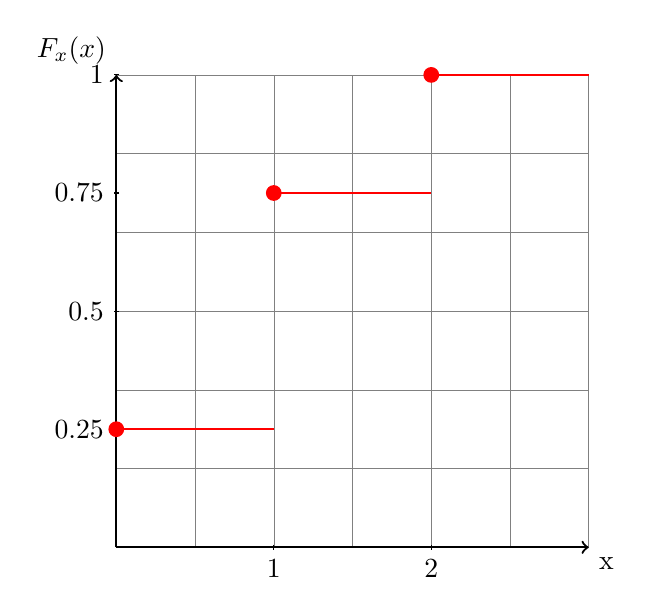
\begin{tikzpicture}
    \draw[step=1cm,gray,very thin] (0,0) grid (6,6);
    \draw[thick,->] (0,0) -- (6,0) node[anchor=north west] {x};
    \draw[thick,->] (0,0) -- (0,6) node[anchor=south east] {$F_x(x)$};
    \foreach \x in {1,2}
        \draw(2*\x,1pt) -- (2*\x,-1pt) node[anchor=north] {$\x$};
    \foreach \y in {0.25,0.5,0.75,1}
        \draw(1pt,6*\y) -- (-1pt,6*\y) node[anchor=east] {$\y$};
    \draw[red,thick] (0,1.5) -- (2,1.5);
    \draw[red,thick] (2,4.5) -- (4,4.5);
    \draw[red,thick] (4,6) -- (6,6);
    \fill[red] (0,1.5) circle (0.1cm);
    \fill[red] (2,4.5) circle (0.1cm);
    \fill[red] (4,6) circle (0.1cm);
\end{tikzpicture}

\subsubsection{Satz 3.2: Eigenschaften von VF} 
Sei X eine ZV und F ihre VF. Dann gilt
\begin{itemize}
    \item[(a)] F ist monoton wachsend.
    \newline Für alle $x,y\in\mathbb{R}$ mit $x<y$ gilt $F(x)\leq F(y)$.
    \item[(b)] $\lim_{x\rightarrow-\infty}F(x)=0, \lim_{x\rightarrow\infty}F(x)=1$
    \item[(c)] F ist rechtsseitig stetig.
    \item[(d)] $P(X>x)=1-F(x), x\in\mathbb{R}$
    \item[(e)] $P((a<X\leq b))= $
    \item[(f)] $P(X<x)=F(x-)$, wobei $F(x-)=lim_{y\rightarrow x}F(y)$ der linksseitige Grenzwert von F an der stelle x ist, d.h., der Grenzwert der Werte $F(y)$ wenn y sich x von links nähert.
    \item[(g)] $P(X=x)=F(x)-F(x-) =$ Sprunghöhe von F an der Stelle X
    \newline Insb.
    \newline
    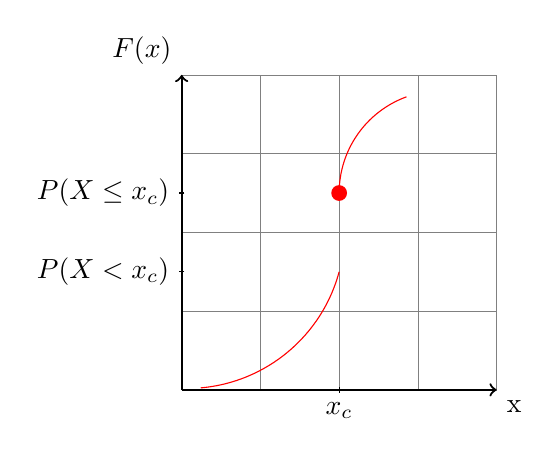
\begin{tikzpicture}
        \draw[step=1cm,gray,very thin] (0,0) grid (4,4);
        \draw[thick,->] (0,0) -- (4,0) node[anchor=north west] {x};
        \draw[thick,->] (0,0) -- (0,4) node[anchor=south east] {$F(x)$};
        \draw(2,1pt) -- (2,-1pt) node[anchor=north] {$x_c$};
        \draw(1pt,1.5) -- (-1pt,1.5) node[anchor=east] {$P(X<x_c)$};
        \draw(1pt,2.5) -- (-1pt,2.5) node[anchor=east] {$P(X\leq x_c)$};
        \fill[red] (2,2.5) circle (0.1cm);
        \draw[red] (2,1.5) arc (-15:-85:2);
        \draw[red] (2,2.5) arc (180:110:1.3);
    \end{tikzpicture}
    \newline $P(X=x)=P(X\leq x_c)-P(X<x_c)$ (s. Sprung in der Grafik)
    \newline $P(X=x)=0 \Leftrightarrow$ F ist stetig an der Stelle X
    \newline $P(X=x)=0$ für alle $x\in\mathbb{R} \Leftrightarrow$ F ist stetig auf $\mathbb{R}$
    \item[(h)] $P(X\geq x)=1-F(x-)$
    \newline $ P(X\leq X \leq b) = F(b)-F(a-), \hspace{15pt} a\leq b$
\end{itemize}

\vspace{6pt}
\noindent\textbf{Beweis:} 
\begin{itemize}
\item[(a),(e)] Für $a<b$ gilt $0\leq P(a<X\leq b) = P(\{X\leq b\}\backslash \{X\leq a\}) = $
    \newline $= P(X\leq b) - P(X\leq a) = F(b) - F(a)$
\item[(b),(c)] Übungsaufgabe 21
\item[(d)] $P(X>x) = P(\{X\leq x\}^c) = 1-P(X\leq x)=1-F(x)$
\item[(f)] $P(X<x)=P(\bigcup_{n=1}^{\infty}\{X\leq x-\frac{1}{n}\})$
    \newline Übungsaufgabe 20 $= \lim_{n\rightarrow\infty}P(X\leq x-\frac{1}{n}) = \lim_{n\rightarrow\infty}F(x-\frac{1}{n}) = F(x-)$
    \newline $\{X\leq x-\frac{1}{n}\}\subset\{X\leq x-\frac{1}{n+1}\}$
\item[(h)] $P(X\leq x) = P(\{X<x\}^c)=1-P(X<x) \fover 1-F(x-)$
    \newline $P(a\leq X\leq b) = P(\{x\leq b\} \backslash \{X<a\}) = P(X\leq b) - P(X<a) = F(b) - F(a-)$.
    \newline Für $a=b=x$ ergibt sich (g).
\end{itemize}

\vspace{6pt}
\noindent\textbf{Bem. 3.2:} Man kann zeigen: 
\begin{itemize}
\item[(a)] Jede Funktion $F:\mathbb{R}\rightarrow\mathbb{R}$, die $(a)-(c)$ aus Satz 3.2 erfüllt, ist die VF einer geeigneten ZV.
\item[(b)] Seien $X$ und $Y$ ZF mit VF $F_x$ und $F_y$. Dann gilt
    \newline $F_x(x)=F_y(x)$ für alle $x\in\mathbb{R} \Leftrightarrow P(X\in B) = P(Y\in B)$ für alle $B\in\mathbb{R}$.
    \newline Falls $F_x(x)=F_y(x)$, dann sagt man \glqq X und Y sind identisch verteilt\grqq.
\end{itemize}

\subsubsection{Diskrete ZV}
\vspace{6pt}
\noindent\textbf{Def. 3.4:} Eine ZV X heißt \textit{diskret}, falls X höchstens abzählbar viele Werte $x_1,x_2,\dots$ annimmt. 
\newline Ist X eine diskrete ZV, dann heißt die durch 
\[f(x)=P(X=x) \hspace{15pt} x\in\mathbb{R},\]
definierte Funktion $f:\mathbb{R}\rightarrow\mathbb{R}$ die \textit{Wahrscheinlichkeitsfunktion} von X.

\vspace{6pt}
\noindent Sei X eine diskrete ZV mit W'funktion f und VF F. Bezeichne die möglichen Werte von X mit $x_1,x_2,\dots$, d.h., 
\[\{x_1,x_2,\dots\}=\{X(a):\omega\in\Omega\}\]
Dann gilt für jedes $B\in\mathbb{R}$,
\[P(X\in B)=P(\bigcup_{x\in B}\{X=x\})=\sum_{x_i\in B}P(X=x)=\sum_{x_i\in B}f(x_i)\]

\begin{align*}
\sum_{x_i\in\mathbb{R}}f(x_i) &= P(X\in\mathbb{R})=1 \\ 
F(x) &= P(X\leq x) = \sum_{x_i\leq x}f(x), \hspace{15pt}x\in\mathbb{R}\\
f(x) &= P(X=x)\hspace{15pt}\eqthreetwog \hspace{15pt} F(x)-F(x-) \hspace{15pt} x\in\mathbb{R}\\
\end{align*}

\vspace{6pt}
\noindent Setze
\[P_x(B)=P(X\in B) \text{ für jedes } B\in\mathbb{R}.\]
Dann ist $P_x$ ein W-Maß auf $\mathbb{R}$, denn:
\begin{itemize}
\item[(i)] $P_x(B)\geq 0$ für alle $B\subset\mathbb{R}$
\item[(ii)] $P_x(\mathbb{R})=P(X\in\mathbb{R})=1$
\item[(iii)] $\sigma$-Additivität
    \newline Seien $B_1,B_2,\dots\subset\mathbb{R}$ paarweise disjunkt
    \newline $\Rightarrow P_x(B_1\cup B_2\cup\dots)=P(X\in B_1\cup B_2\cup\dots) = P(\{X\in B_1\}\cup\{X\in B_2\}\cup\dots)$
    \newline $ \eqsigmaadd \hspace{12pt}\sum_{i}P(X\in B_i)=\sum_{i}P_x(B_i)$.
\end{itemize}
Das W-Maß $P_x$ heißt die Verteilung von X.

\subsubsection{Stetige ZV}
\vspace{6pt}
\noindent\textbf{Def. 3.5:} Eine ZV X heißt \textit{stetig}, falls es eine Funktion $f:\mathbb{R}\rightarrow\mathbb{R}$ gibt, so dass 
\begin{align*}
f(x) &\geq 0 \hspace{15pt}\forall x\in\mathbb{R},\\
\int_{-\infty}^{\infty}f(x)dx &= 1 \\
\text{und}\hspace{20pt}P(X\leq x) &= \int_{-\infty}^{\infty}f(u)du \hspace{15pt}\forall x\in\mathbb{R}.
\end{align*}
F heißt \textit{Dichte} oder \textit{Wahrscheinlichkeitsdichte} von X.

\vspace{6pt}
\noindent Sei X eine stetige ZV mit Dichte f und VF F
\newline $\rightarrow$ F ist stetig $\hspace{12pt}\impthreetwog\hspace{12pt} P(X=x)=0$ für alle $x\in\mathbb{R}$.
\newline $\Rightarrow$ Für $a\leq b$ gilt
\begin{align*}
P(a\leq X\leq b) &= P(X=a) + P(a<X<b) + P(X=b) = P(a<X<b)\\
&= P(a\leq X<b) = P(a<X\leq b) = F(b)-F(a)\\
&= \int_{-\infty}^{a}f(x)dx - \int_{-\infty}^{b}f(x)dx = \int_{a}^{b}f(x)dx\\
\end{align*}

\noindent Ist die Dichte f an der Stelle $x_c$ stetig, so gilt 
\[F'(x_c)=f(x_c)\]
f lässt sich aus F gewinnen.

\subsection{Beispiele diskreter Verteilungen}
\noindent\textit{Diskrete Verteilungen}, d.h. Verteilungen von diskreten ZV
\newline Einfachster Fall: $\exists a\in\mathbb{R}$ mit $P(X=a)=1$.

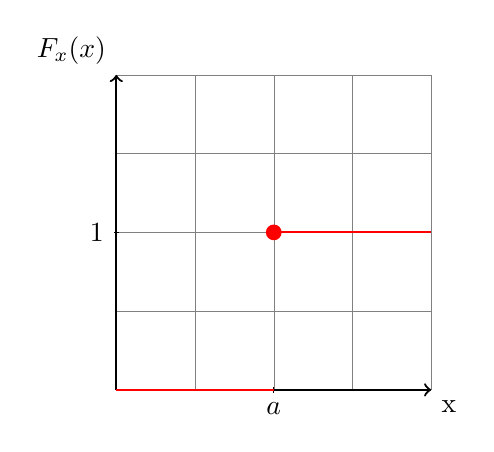
\begin{tikzpicture}
        \draw[step=1cm,gray,very thin] (0,0) grid (4,4);
        \draw[thick,->] (0,0) -- (4,0) node[anchor=north west] {x};
        \draw[thick,->] (0,0) -- (0,4) node[anchor=south east] {$F_x(x)$};
        \draw(2,1pt) -- (2,-1pt) node[anchor=north] {$a$};
        \draw(1pt,2) -- (-1pt,2) node[anchor=east] {$1$};
        \fill[red] (2,2) circle (0.1cm);
        \draw[red,thick] (0,0) -- (2,0);
        \draw[red,thick] (2,2) -- (4,2);
\end{tikzpicture}

\subsubsection{Bernoulli-Verteilung}
\noindent Eine ZV X, die nur die Werte 0 und 1 annimmt mit 
\[P(X=1)=p, P(X=0)=1-p\]
heißt \textit{Bernoulli-verteilt} mit Parameter p.
\newline X wird auch als Bernoulli-Variable bezeichnet. $(0\leq p \leq 1)$
\newline Bez. X$\sim$Ber(p).

\vspace{6pt}
\noindent Sei A ein Ereignis. Die Indikatorfunktion $I_A$ von A (oder Indikatorvariable) ist definiert durch
\begin{equation*}
    I_A(\omega)=\begin{cases}
        1, & \omega\in A\\
        0, & \omega\in A^c\\
    \end{cases}
\end{equation*}

\noindent Also
\newline $I_A(\omega)=1 \Leftrightarrow$ A tritt ein
\newline $X=I_A$ ist eine Bernoulli-Variable mit Parameter p=P(A).
\newline Man sagt oft, 
\begin{align*}
    \text{Erfolg tritt ein, falls } & X(\omega)=1\\
    \text{Misserfolg tritt ein, falls } & X(\omega)=0\\
\end{align*}

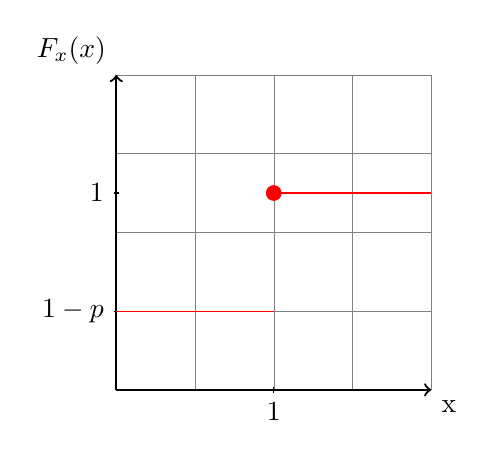
\begin{tikzpicture}
        \draw[step=1cm,gray,very thin] (0,0) grid (4,4);
        \draw[thick,->] (0,0) -- (4,0) node[anchor=north west] {x};
        \draw[thick,->] (0,0) -- (0,4) node[anchor=south east] {$F_x(x)$};
        \draw(2,1pt) -- (2,-1pt) node[anchor=north] {$1$};
        \draw(1pt,1) -- (-1pt,1) node[anchor=east] {$1-p$};
        \draw(1pt,2.5) -- (-1pt,2.5) node[anchor=east] {$1$};
        \fill[red] (2,2.5) circle (0.1cm);
        \draw[red] (0,1) -- (2,1);
        \draw[red] (2,2.5) -- (4,2.5);
\end{tikzpicture}

\subsubsection{Binomialverteilung}
\noindent Seien $X_1,\dots,X_n$ unabhängig und jeweils $~Ber(p)$ (Erfolgsw'keit jeweils p).
\newline Anzahl der Erfolge 
\[S_n:= X_1+\dots+X_n\]
Bsp.: n Münzwürfe
\begin{equation*}
    X_i=\begin{cases}
        1, & \text{im i-ten Wurf K}\\
        0, & \text{im i-ten Wurf Z}\\
    \end{cases}
    S_n = \text{Anzahl der K-Würfe}
\end{equation*}
$S_n$ = Anzahl der K-Würfe $\Rightarrow$ Mögliche Werte von $S_n:0,1,\dots,n.$ $P(S_n=k)=?$
\newline Da $X_1,\dots,X_n$ unabhängig sind, 
\begin{align*}
   & P(X_1=1,\dots,X_k=1, X_{k+1}=0,\dots,X_n=0)\\
   =& P(X_1=1)\cdot\dots\cdot P(X_k=1)\cdot P(X_{k+1}=0)\cdot\dots\cdot P(X_n=0)\\
   =& p^k \cdot q^{n-k} \hspace{15pt} (q:=1-p)
\end{align*}

\noindent $\rightarrow$ hängt nur ab von der Anzahl der vorgegebenen Einsen, nicht von deren Position. Also
\[P(S_n=k)=p^k \cdot q^{n-k}\]
\glqq Anzahl der Möglichkeiten, aus n Versuche k anzugeben, bei denen Erfolg eintreten soll\grqq\
\[\Rightarrow P(S_n=k)=\binom{n}{k}\cdot p^k\cdot q^{n-k}, k=0,1,\dots,n\]
wobei $\binom{n}{k}=\frac{n!}{k!(n-k!)}$ (Binomialkoeffizient).

\noindent Insb. $P(S_n=0)=\binom{n}{0}\cdot p^0\cdot q^n=q^n, P(S_n=1)=\binom{n}{n}\cdot p^n\cdot q^0=p^n$.
\newline $S_n$ heißt \textit{binomialverteilt} mit Parametern n(\# Versuchen) und p(Erfolgsw'keit).
\newline Bez. $S_n\sim$Bin(n,p)

\vspace{6pt}
\noindent\textbf{Bsp. 3.6:} Wie groß ist die W'keit, dass von 5 E-Mails höchstens eine Spam ist, wenn bei jeder E-Mail die W'keit für Spam $\frac{1}{3}$ ist?
\newline X=Anzahl der Spam E-Mails $\sim$Bin$(5,\frac{1}{3})$
\begin{align*}
P(X\leq 1) &= P(X=0)+P(X=1)\\
&= \binom{5}{0}\cdot (\frac{1}{3})^0\cdot (\frac{2}{3})^5 + \binom{5}{1}\cdot (\frac{1}{3})^1\cdot (\frac{2}{3})^5\\
&= \frac{2^5}{3^5}+\frac{5!}{1!4!}\cdot
\end{align*}

\subsubsection{Geometrische Verteilung}
Seien $X_1,X_2,\dots$ unabh., $\sim$Ber(p), $0<p\leq 1$
\newline $X_i=1 \leftrightarrow$ Erfolg im i-ten Versuch.
\newline T = Anuahl der Versuche bis zum ersten Erfolg (einschließlich)
\[P(T=1)=P(X_1=1)=p\]
\newline Für $k\geq 2$ ist
\begin{align*}
P(T=k) &= (X_1=0,\dots,X_{k-1}=0,X_k=1)\\
&= P(X_1=0)\cdot\dots\cdot P(X_{k-1}=0)\cdot P(X_k=1) = (1-p)^{k-1}\cdot p
\end{align*}
Mit $q=1-p$ also 
\[P(T=k)=q^{k-1}\cdot p, k=1,2,\dots\]
Bez. T$\sim$Geo(p) Geometrische Verteilung mit Parameter $0<p\leq1$.
\newline Beachte
\[\sum_{k=1}^{\infty}q^{k-1}\cdot p = p(1+q+q^2+\dots)=p\cdot \frac{1}{1-q}= \frac{p}{p}=1\]

\subsubsection{Poisson-Verteilung}
Eine ZV X heißt \textit{Poisson-verteilt} mit Parameter $\lambda >0$, falls
\[P(X=k)=\frac{\lambda^k}{k!}\cdot e^{-\lambda}, \hspace{15pt} k=0,1,2,\dots\]
Bez. X$\sim$Poi$(\lambda)$.
\newline Beachte
\[\sum_{k=0}^{\infty}\frac{\lambda^k}{k!}\cdot e^{-\lambda} = e^{-\lambda}\cdot \sum_{k=0}^{\infty}\frac{\lambda^k}{k!} = e^{-\lambda}\cdot e^\lambda = 1\]
über die Taylor-Reihe für $e^\lambda$.

\noindent Anwendung der Posison-Verteilung zu Approximation einer Binomialverteilung. 
\newline Sei X$\sim$Bin(n,p). Ist n \glqq groß\grqq\ und p \glqq klein\grqq\, etwa $n\geq50,p\leq\frac{1}{10}$ und $np\leq10$, dann
\[P(X=k)\approx P(Y=k), \text{wobei} Y~Poi(n,p)\]

\vspace{6pt}
\noindent\textbf{Bsp. 3.7:} 
Ein Callcenter erhält in jeder Sekunde mit W'keit 0,001 einen Anruf. 
Anrufe erfolgen unabhängig.

\noindent $X=$ Anzahl der Anrufe in einer Stunde
\newline $\sim$Bin(n,p) mit $n=3600$ und $p=0,001$
\newline $\Rightarrow$ Poisson-Approximation [$n\geq 50, p\leq\frac{1}{10}, np=2,6\leq10$]
\newline Approximiere Bin(n,p) durch Poi$(\lambda)$ mit $\lambda=np=3,6$.
\[P(X=k)=\frac{\lambda^k}{k!}\cdot e^{-\lambda}=P(Y=k) \hspace{15pt}\text{wobei } Y~Poi(\lambda)\]

\begin{center}
\begin{tabular}{c|c c c}
    k & 0 & 1 & 2 \\
    \hline
    $P(X=k)$ & .02727 & .09829 & .1770 \\
    $P(Y=k)$ & .02732 & .09837 & .1771 \\
\end{tabular}
\end{center}

\subsubsection{Hypergeometrische Verteilung}
Warenlieferung enthalten N Stücken, davon M defekt (N-M intakt)
\newline Es werden n Stücke ohne Zurücklegen zufällig gezogen, wobei $n\leq N$.



\end{document}

